%%%%%%%%%%%%%%%%%%%%%%%%%%%%%%%%%%%%%%%%%%%%%%%%%%%%%%%%%%%%%%%%%%%%%%%%%%%%%%%%
%2345678901234567890123456789012345678901234567890123456789012345678901234567890
%        1         2         3         4         5         6         7         8

%\documentclass[letterpaper, 10 pt, conference]{ieeeconf} % Comment this line out
                                                          % if you need a4paper
\documentclass[a4paper, 10pt, conference]{ieeeconf}       % Use this line for a4
                                                          % paper

\IEEEoverridecommandlockouts                              % This command is only
                                                          % needed if you want to
                                                          % use the \thanks command
\overrideIEEEmargins
% See the \addtolength command later in the file to balance the column lengths
% on the last page of the document

\usepackage{graphicx}
\graphicspath{{../data/}}

% The following packages can be found on http:\\www.ctan.org
%\usepackage{graphics} % for pdf, bitmapped graphics files
%\usepackage{epsfig} % for postscript graphics files
%\usepackage{mathptmx} % assumes new font selection scheme installed
%\usepackage{times} % assumes new font selection scheme installed
%\usepackage{amsmath} % assumes amsmath package installed
%\usepackage{amssymb}  % assumes amsmath package installed

\title{\LARGE \bf
  ROS : Robotics Operating System
}

%\author{ \parbox{3 in}{\centering Huibert Kwakernaak*
%         \thanks{*Use the $\backslash$thanks command to put information here}\\
%         Faculty of Electrical Engineering, Mathematics and Computer Science\\
%         University of Twente\\
%         7500 AE Enschede, The Netherlands\\
%         {\tt\small h.kwakernaak@autsubmit.com}}
%         \hspace*{ 0.5 in}
%         \parbox{3 in}{ \centering Pradeep Misra**
%         \thanks{**The footnote marks may be inserted manually}\\
%        Department of Electrical Engineering \\
%         Wright State University\\
%         Dayton, OH 45435, USA\\
%         {\tt\small pmisra@cs.wright.edu}}
%}

\author{
  Weipeng He
%\thanks{$^{1}$W. He is with Department of Informatics,
%        University of Hamburg, Vogt-K\"olln-Stra\ss e 30, Germany, 
%        {\tt\small 2he at informatik.uni-hamburg.de}}%
\\ Department of Informatics\\ University of Hamburg \\ {\tt\small 2he@informatik.uni-hamburg.de}
}

\begin{document}

\maketitle
\thispagestyle{empty}
\pagestyle{empty}

%%%%%%%%%%%%%%%%%%%%%%%%%%%%%%%%%%%%%%%%%%%%%%%%%%%%%%%%%%%%%%%%%%%%%%%%%%%%%%%%
\begin{abstract}
  ROS is
\end{abstract}


%%%%%%%%%%%%%%%%%%%%%%%%%%%%%%%%%%%%%%%%%%%%%%%%%%%%%%%%%%%%%%%%%%%%%%%%%%%%%%%%
\section{INTRODUCTION}

Software system for robots is difficult to develop because of the diversity of hardware and fast growing of its scale. Different research groups write their software for various types of robots, hardware and drivers. The software architectures they chose also differ. All these facts make the codes in robotics hard to reuse. Because of low reusability, researchers, in some cases, need to write the codes from scratch. Furthermore, the low reusability makes it hard to reproduce the experimental results from different groups.

Robot Operating System (ROS) is a project that promotes the code reuse in robotics research\cite{quigley_ros:_2009}. ROS is an open-source, meta-operating system for robots. It provides the services including hardware abstraction, low-level device control, implementation of commonly-used functionality, message-passing between processes, and package management. It also provides tools and libraries for obtaining, building, writing, and running code across multiple computers. Last but not least, ROS is supported by a open-source community (ROS.org), which is a platform for researchers to use for collaborating.

ROS was started from 2007, and now it is widely used in research and industry of robotics. Originally, it was under the name switchyard by the Stanford Artificial Intelligence Laboratory in support of the Stanford AI Robot (STAIR) project. From 2008, its development continues primarily at Willow Garage, with more than twenty institutions collaborating in a federated development model. ROS has been released several times under different distribution names. The latest stable distribution release is ``ROS Groovy Galapagos'' on December 31, 2012\cite{_documentation_2013}.

Although the latest release of ROS is targeted at Ubuntu, it also works on other linux distributions as well as Mac OS X, Android, and Windows. ROS programs can be developed in multiple programming languages, that are C++, Python and Lisp. More importantly, ROS supports more than 80 diffrent kinds of robots. The popular robots, that are PR2, Care-O-bot 3, iRobot Create, Aldebaran Nao are all included.

Previously, there were other robotics software frameworks used in academia and industry\cite{kramer_development_2007}. Each framework was designed for some special robots or for few special tasks. Among those frameworks, Player/Stage\cite{collett_player_2005} is most similar to ROS. It is also an open-source project, and offers modules for freqently-used robotics applications. Player/Stage fits for simple, non-articulated mobile platforms. ROS, however, is better at dealing with complex mobile manipulation platforms. Furthermore, ROS offers more implementations of robotics-related algorithms.

In later sections of this paper, we will introduce the design goals, software structure and the community management of ROS. 

\section{Design goals}




\section{Software Structure}

\textbf{Software Structure}
\textit{ROS Computation Graph}

\begin{itemize}
  \item The ROS runtime "graph" is a peer-to-peer network of processes using the ROS communication infrastructure.
\end{itemize}
\begin{center}
  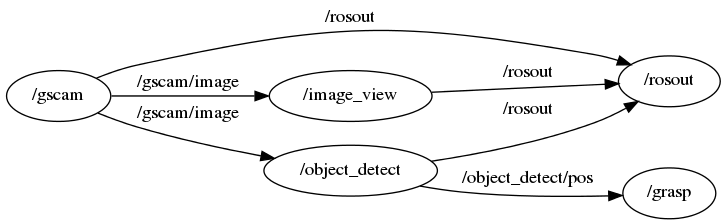
\includegraphics[width=\textwidth]{comp_graph}
\end{center}




\textbf{Software Structure}
\textit{Node and Master}

\begin{itemize}
  \item Nodes are processes that perform computation. 
  \item ROS is designed to be modular at a fine-grained scale. Robot control system will usually comprise many nodes.
  \item For example, one node controls a laser range-finder, one node controls the wheel motors, one node performs localization, one node performs path planning, one node provides a graphical view of the system, and so on.
  \item Nodes get to know each other via roscore (master).
\end{itemize}

\begin{center}
  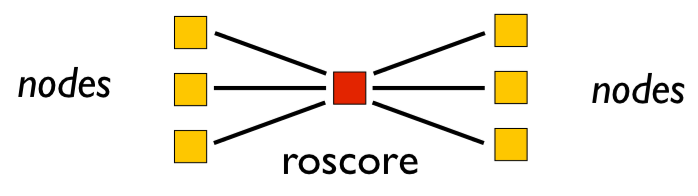
\includegraphics[width=.6\textwidth]{nodes}
\end{center}




\textbf{Software Structure}
\textit{Message}

\begin{itemize}
  \item Nodes communicate with each other by passing messages.
  \item A message is simply a data structure, comprising typed fields. 
  \item Standard primitive types (integer, floating point, boolean, etc.) are supported, as are arrays of primitive types. 
  \item Messages can include arbitrarily nested structures and arrays (much like C structs).
\end{itemize}



\textbf{Software Structure}
\textit{Message example}

\begin{itemize}
  \item sensor\_msg/Image
\end{itemize}

Header header \\
~  uint32 seq \\
~  time stamp \\
~  string frame\_id \\
uint32 height \\
uint32 width \\
string encoding \\
uint8 is\_bigendian \\
uint32 step \\
uint8[] data



\textbf{Software Structure}
\textit{Topic}

\begin{itemize}
  \item Topic is a mechanism to send messages from a node to one or more nodes.
  \item Follows a publisher-subscriber design pattern.
  \item Publisher is the node which send messages to the topic.
  \item Subscribers are the nodes which get called whenever a message is published.
  \item Example : Camera publishing images.
\end{itemize}

\begin{center}
  
\includegraphics[width=.6\textwidth]{topic}
\end{center}




\textbf{Software Structure}
\textit{Service}

\begin{itemize}
  \item Service is a mechanism for a node to send a request to another node and receive a response in return.
  \item Follows a request-response design pattern.
  \item A service is called with a request message, and in return, a response message is returned.
  \item Example : Request the camera to tilt.
\end{itemize}

\begin{center}
  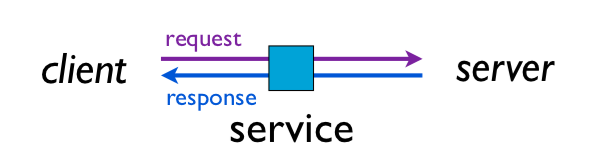
\includegraphics[width=.6\textwidth]{service}
\end{center}



\textbf{Software Structure}
\textit{File system Hierarchy}

\begin{itemize}
  \item Release : collection of stacks and packages.
  \begin{itemize}
    \item Fuerte
  \end{itemize}
  \item Stacks : a full application suite.
  \begin{itemize}
    \item geometry
  \end{itemize}
  \item Package : software to solve a specific task.
  \begin{itemize}
    \item tf
  \end{itemize}
  \item Node : an executable.
  \begin{itemize}
    \item tf\_echo
  \end{itemize}
\end{itemize}



\section{Community Management}

\textbf{Community}
\textit{Software Distribution}

\begin{itemize}
  \item ROS code is maintained in a decentralized federation of repositories.
  \begin{itemize}
    \item The core repository : ros-pkg;
    \item 94 repositories in other institutions;
    \item 14 personal repositories.
  \end{itemize}
  \item Easy to contribute.
  \begin{itemize}
    \item Host their code (and documents) in their own repository.
    \item SourceForge.net, Google Code and GitHub.
    \item Register at ros.org.
  \end{itemize}
  \item Easy to search software.
  \begin{itemize}
    \item Search across the federation of repositories is possible.
    \item ros.org keeps tracks of updates of all repositories and generates index.
    \item Documentation and tutorials are also updated automatically.
  \end{itemize}
\end{itemize}




\textbf{Community}

\begin{itemize}
  \item ROS Answers.
\end{itemize}
\begin{center}
  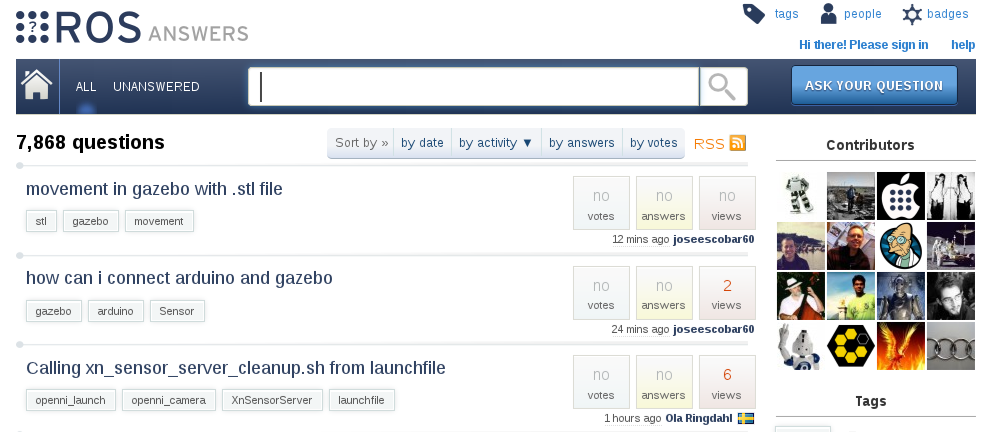
\includegraphics[width=\textwidth]{ros_answers}
\end{center}


\section{Conclusion}

\textbf{Conclusion}

\begin{itemize}
  \item ROS defines a standard for the communicate mechanisms and protocols between robot components.
  \item ROS provides libraries for various functions.
  \item ROS contains utility tools to help development.
  \item ROS promotes code sharing and reuse.
\end{itemize}

\textbf{Questions?}
Thanks!

\bibliography{ref}
\bibliographystyle{plain}  

\end{document}
